\section{Introduction}
\label{sec:introduction}

\subsection{Industrial Context and the Skip Dilemma}
Modern recommender systems for audio streaming platforms (e.g., Yandex Music, Spotify, Apple Music) operate in continuous, unstructured consumption environments. Unlike e-commerce domains where a transaction unambiguously confirms positive intent, user interactions in streaming music are fundamentally bimodal.

Analysis of interaction logs on the large-scale Yandex Music dataset (\textbf{Yambda-50M})~\cite{ploshkin2025yambda,matveev2026session} reveals that \textbf{30\% to 35\%} of all recorded events represent immediate skips: the continuous listening duration is less than 30 seconds (or even 0.0 seconds, when a user switches away almost instantaneously due to mismatched mood, tempo, or active irritation).

\begin{figure}[!htbp]
    \centering
    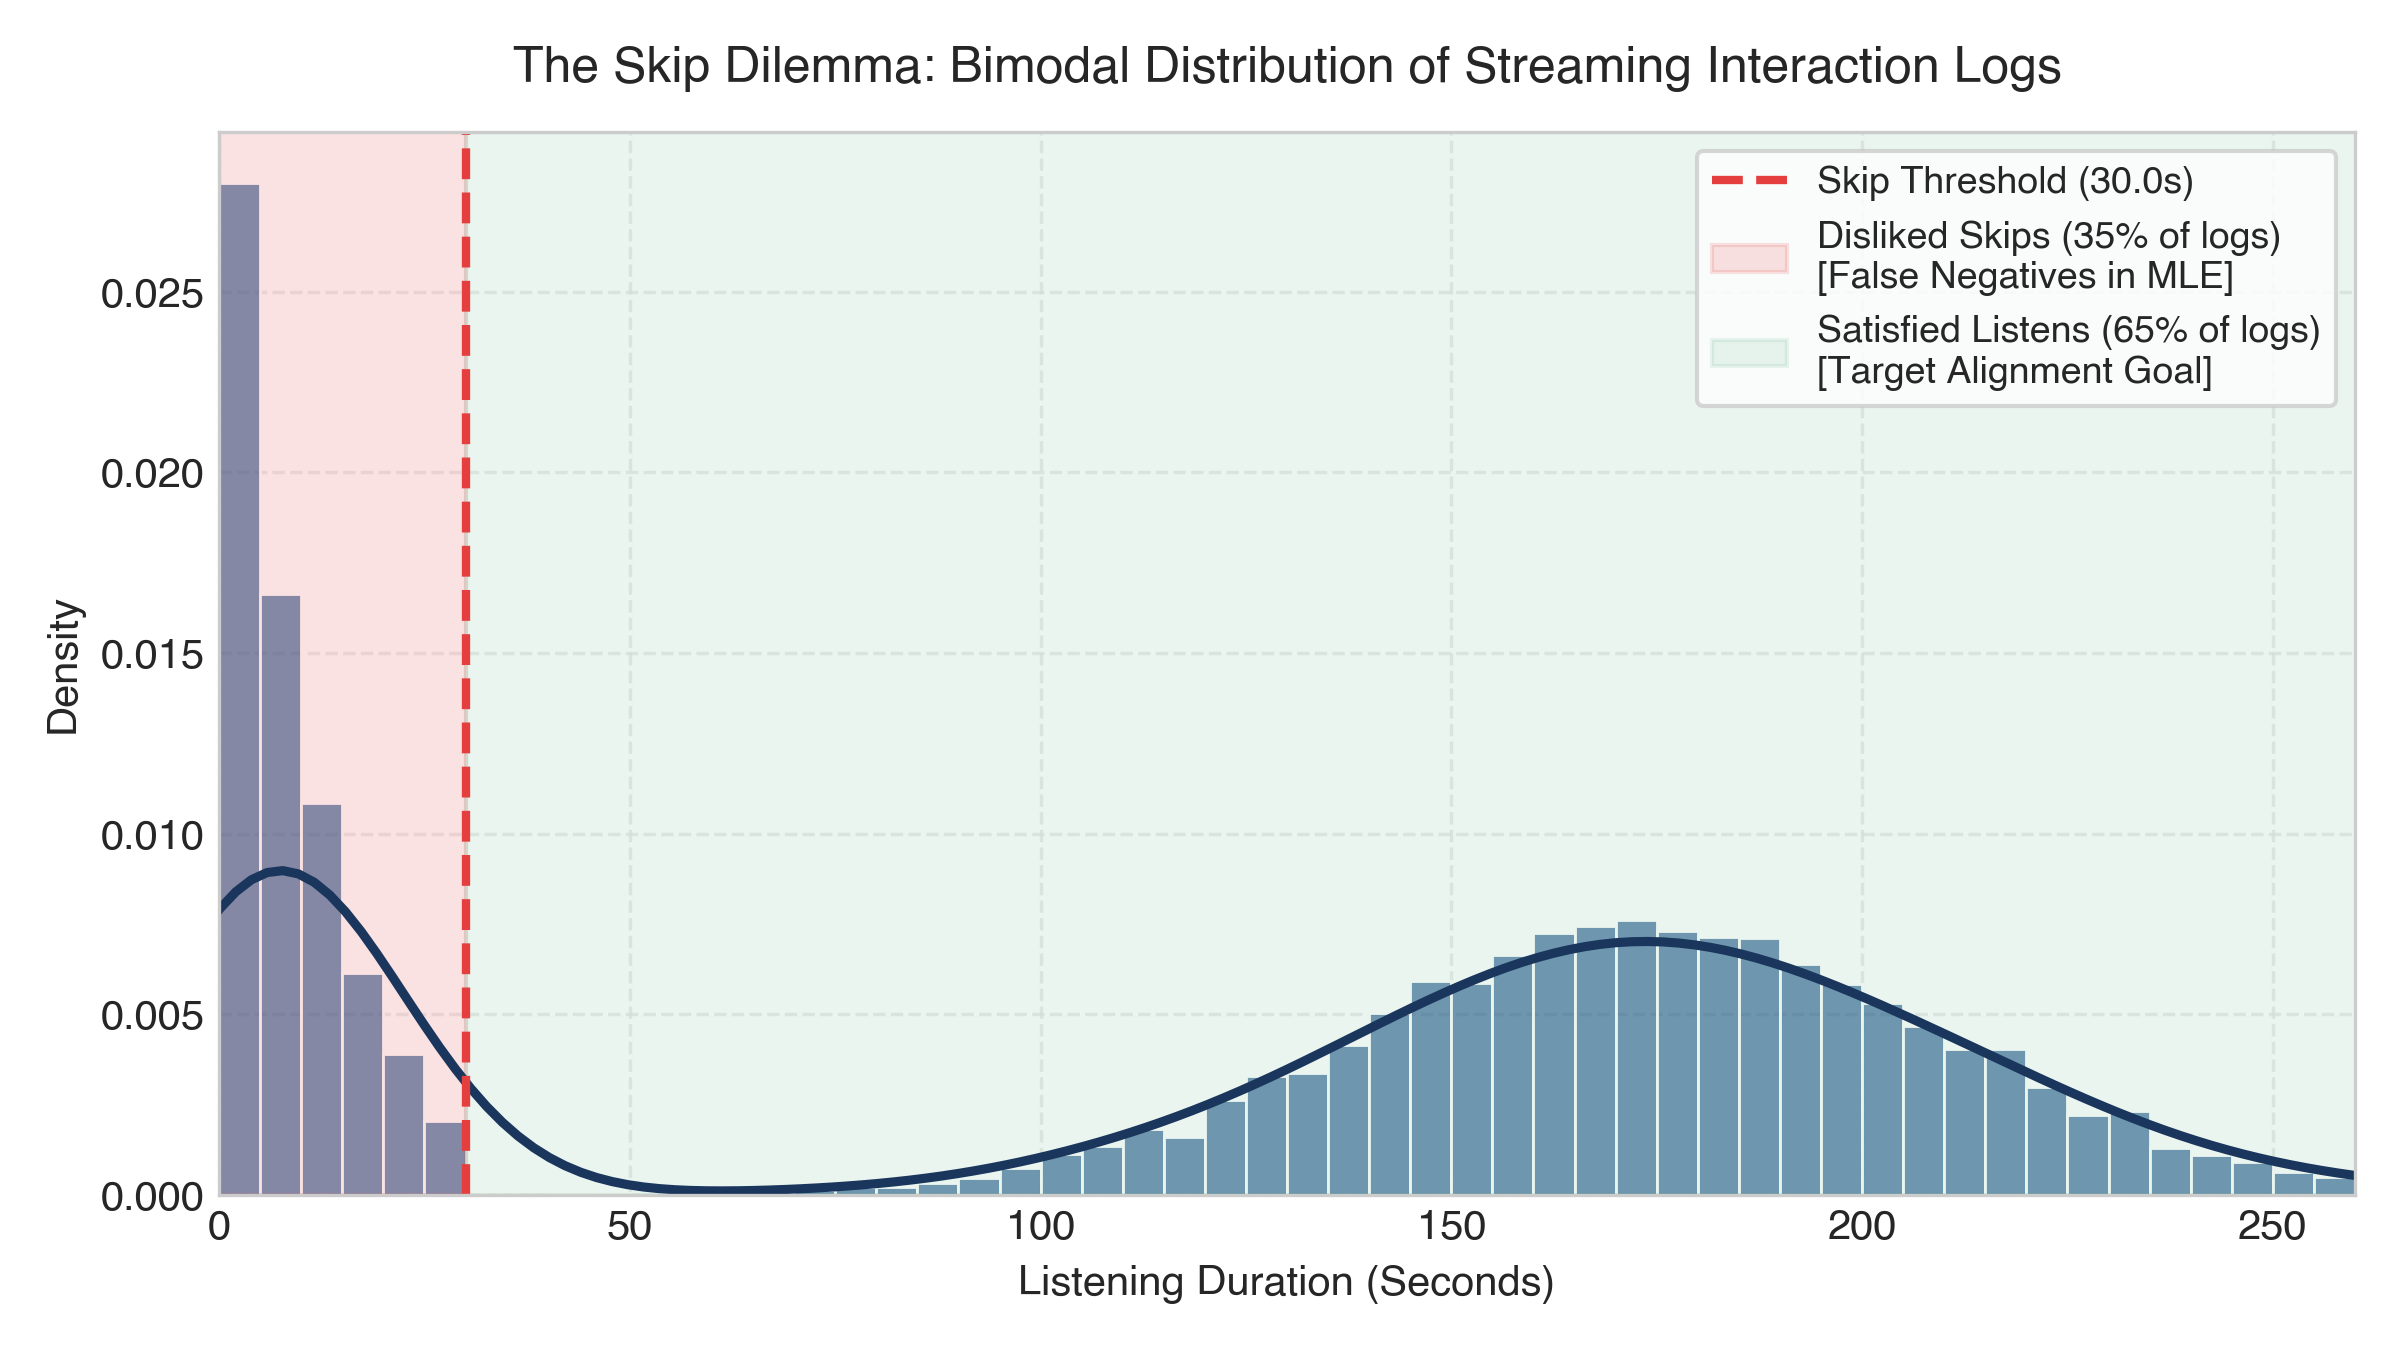
\includegraphics[width=0.78\textwidth]{fig1_the_skip_dilemma.png}
    \caption{\textbf{The Skip Dilemma in music streaming logs.} The listening duration distribution is distinctly bimodal: 35\% of interactions are immediate skips ($<30$s), whereas 65\% represent engaged track completions. Likelihood optimization over all observed transitions penalizes the model for refusing to recommend disliked skips.}
    \label{fig:skip_dilemma}
\end{figure}

\subsection{The False Negative Trap in Likelihood Optimization (MLE)}
The standard paradigm for training sequential recommender systems (e.g., SASRec~\cite{kang2018self} and generative autoregressive transformers~\cite{petrov2024aligning}) formulates recommendation as Next-Item Prediction via cross-entropy loss minimization (Maximum Likelihood Estimation, MLE):
\begin{equation}
    \mathcal{L}_{\text{MLE}}(\theta) = - \sum_{t=1}^{T} \log \pi_\theta(a_t \mid s_{<t}),
    \label{eq:mle_loss}
\end{equation}
where $s_{<t} = (a_1, \dots, a_{t-1})$ denotes the user's sequential history, and $a_t$ is the ground-truth next track logged in the session.

This framing introduces a fundamental conceptual misalignment:
\begin{enumerate}
    \item \textbf{Penalizing Correct Avoidance (False Negative Problem):} If a user initiated track $a_t$ and abandoned it within 1--2 seconds due to frustration, $\mathcal{L}_{\text{MLE}}$ nonetheless penalizes the recommender whenever the model assigns a low posterior probability to $a_t$.
    \item \textbf{Blindness to Consumption Quality:} The model is trained to reproduce historical click trajectories rather than maximize satisfaction, engagement, and uninterrupted listening time~\cite{matveev2026session}.
    \item \textbf{Popularity Bias Amplification:} Supervised training on raw streaming logs forces autoregressive models to over-exploit safe, high-frequency pop tracks, severely compressing catalog diversity~\cite{petrov2024aligning}.
\end{enumerate}

\subsection{Research Questions}
To resolve the skip dilemma, this paper investigates the alignment of a causal language model with user satisfaction using Reinforcement Learning and direct preference optimization. We formulate five core research questions:
\begin{itemize}
    \item \textbf{RQ1 (Policy Behavior and Dynamics):} How does direct preference optimization (DPO) reshape the model's posterior probability distribution compared to MLE, and how rapidly does the implicit reward margin converge?
    \item \textbf{RQ2 (Alignment Tax and Pareto Trade-Off):} Does offline reward alignment degrade next-item ranking accuracy, and can an auxiliary SFT anchor ($\mathcal{L}_{\text{SFT}}$) eliminate this degradation?
    \item \textbf{RQ3 (Catalog Health and Long-Tail Discovery):} Does the aligned policy collapse into a narrow subset of ubiquitous pop hits, or does it stimulate discovery of high-retention long-tail tracks?
    \item \textbf{RQ4 (Autoregressive Queue Robustness):} How does the aligned policy perform when unrolled autoregressively for 5 consecutive steps without intervening user feedback under exposure bias?
    \item \textbf{RQ5 (Long-Term Proxies and Online A/B Validation):} How can session-level offline rewards be translated into long-term retention metrics (e.g., D7/D30 retention) in an industrial A/B testing design?
\end{itemize}

\subsection{Summary of Contributions}
The key scientific and engineering contributions of this work are as follows:
\begin{enumerate}
    \item \textbf{Multi-Paradigm Comparative Study:} On the unified industrial Yambda-50M dataset, we benchmark four distinct paradigms: a Causal GPT-2 backbone, two-stage re-ranking via a state-action critic $Q(s, a)$, Actor-Critic PPO~\cite{schulman2017proximal}, and end-to-end Direct Preference Optimization (DPO)~\cite{rafailov2023direct}.
    \item \textbf{Demonstration of Zero Alignment Tax:} We show that adding an auxiliary SFT anchor ($\gamma=0.10$) preserves the underlying semantic coherence of the session, completely avoiding the alignment tax and achieving statistically significant ranking order gains (+1.32\% relative NDCG@10 gain, $p = 0.0366$; +1.69\% relative MRR gain, $p = 0.0260$, with +0.15\% HR@10 gain).
    \item \textbf{Empirical Audit of Reward Formulations:} We investigate binary duration thresholds, continuous completion ratios, and composite repetition-penalized rewards, identifying margin-threshold filtering as the most robust choice.
    \item \textbf{Catalog Health Expansion:} We demonstrate that DPO reduces Spearman rank correlation with popularity by 13.4\% while exposing users to +197 additional unique long-tail tracks.
\end{enumerate}
